\section{Overview}
...

Android mobile devices use Content Providers in order to allow applications (or apps in short), installed on the device, access to user data. Android's permission mechanism controls whether such an access will be allowed or not. However, the current permission model for Android is a ``all or nothing'' model. The user has to either accept all the permissions that the app requests or they cannot install the app. Such a model is overtly restrictive and does not allow the possibility of execution time permission granting. It also does not allow the user to restrict the data or allow data access based on contextual situations. Current generation of mobile devices are capable of collecting a lot of user information using in-built sensors or by accessing user personal contacts, calendar, emails and messages. In such a situation it has become necessary that user have more control over their data. There needs to be a better way of controlling such data. In this paper we implement a new privacy aware middle-ware, SPrivacy. SPrivacy allows the users to dynamically control the data that an app is allowed to access. 

Traditional solution(s) for controlling user data privacy on mobile devices have focused on two techniques:
\begin{enumerate}
	\item Make changes to the mobile operating system and control how data flows from the creator to the consumer of the data on the device. This is done by creating custom ROMs or mobile operating systems and modifying the APIs in the custom operating system to achieve the goal mentioned before.
	\item Obtain elevated privileges from the operating system in order to control how the data flows. In this mechanism an app is installed on the device with ``root'' privileges on the device so that the app is able to modify the behavior operating system APIs as per its needs.
\end{enumerate}

We argue that both these techniques potentially create loopholes which might be used by a malicious app towards its own untoward actions. Our proposed mechanism allows us to have no changes on the operating systems but at the same time allows us to control the data that an app can access on the device. We achieve this by implementing SPrivacy which is a middle-ware that is capable, based on a list of settings and a URI redirection mechanism, of controlling the data app(s) get. In our mechanism we take apps from the Android app market and modify the Content Provider URIs they use in order to ensure they call our middle-ware instead. Our middle-ware on then determines if the app will be given access to the data or not.

\section{System Design and Architecture}

system design

\begin{figure}[!htb]
	\centering
	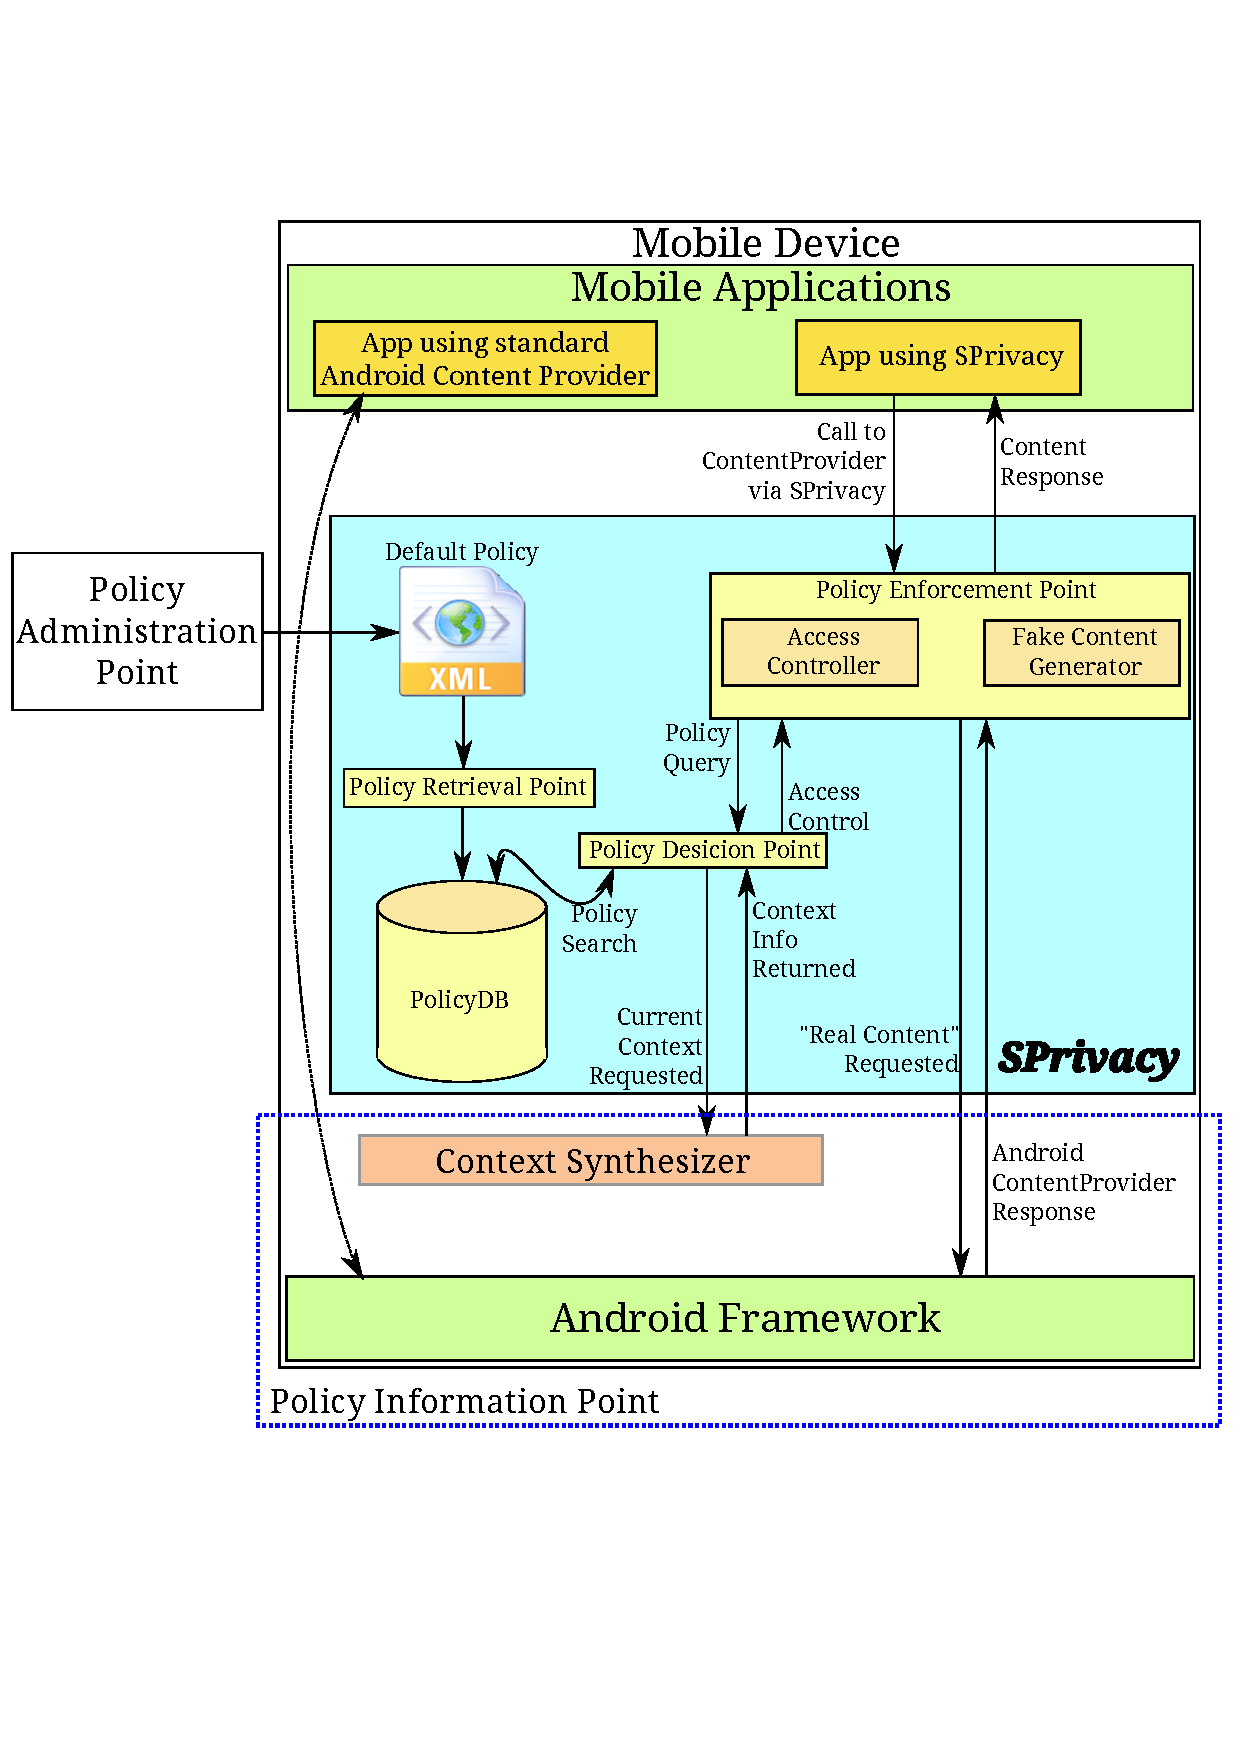
\includegraphics[width=0.9\columnwidth]{images/architecture}
	\caption{High-level architecture of our system.}
	\label{fig:architecture}
\end{figure}
